

\begin{multicols}{2}
\begin{justify}
\begin{flushleft}
    

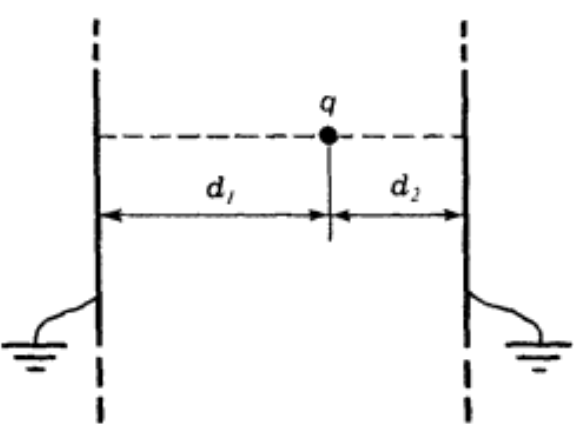
\includegraphics[scale=0.6]{image.png}

\textbf{Рис. 3.}\\
таких методов, основанный на теореме (или принципе) взаимности.
\end{flushleft}



В чем заключается сущность этой теоремы? Ее можно сформулировать так: \textit{если в системе из n проводников проводники, несущие заряды $q_1, q_2, ... , q_n,$ имеют потенциалы $\varphi_1, \varphi_2, ..., \varphi_n$ соответственно, а при зарядах $q'_1, q'_2, ... , q'_n,$ потенциалы проводников равны $\varphi'_1, \varphi'_2, ..., \varphi'_n$, то справедливо равенство}
\[\sum_{i=1}^{n} q_i \varphi'_i = \sum_{i=1}^{n} q'_i \varphi_i. \eqno(1)\]

\begin{flushleft}
Покажем, что это действительно так.
\end{flushleft}

Согласно принципу суперпозиции потенциалы проводников находятся в линейной зависимости от зарядов. Или, наоборот, заряды на проводниках линейно зависят от потенциалов. Рассмотриим сначала частный случай --- внутри заземленной проводящей поверхности находятся два заряженных проводника $1$ и $2$ (рис. 4). Соединим второй проводник с заземленной поверхностью, тогда потенциал этого проводника обратится в нуль (см. рис. 4. \textit{а}). Потенциал первого проводника обозначим через $\varphi_1$. Заряды на каждом из проводников должны быть пропорциональны $\varphi_1$, т.е.
\[ \Delta q_1 = C_1_1 \varphi_1 \textrm{ и } \Delta q_2 = C_2_1 \varphi_1. \eqno(2)\]
\end{justify}
\begin{justify}
    Здесь $\Delta q_1$ и $\Delta q_2$ --- заряды на первом и втором проводниках соответственно, а $C_1_1$ и $C_2_1$ --- постоянные величины, называемые коэффициентами емкости и зависящие от формы и взаимного расположения проводников. $C_1_1$ и $C_2_1$ характеризуют заряды первого
\end{justify}

\columnbreak
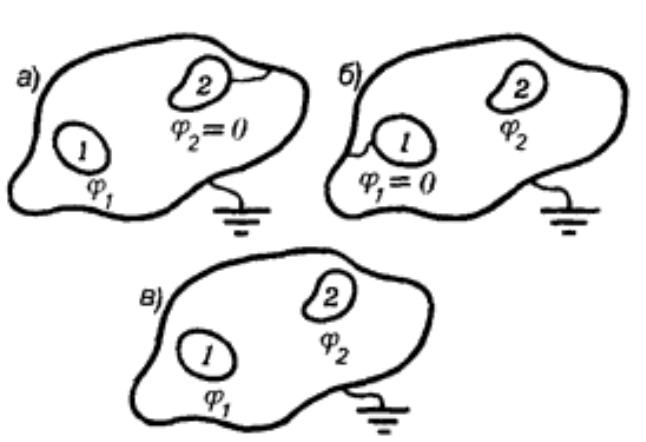
\includegraphics[scale=0.6]{image2.png}

\textbf{Рис. 4.}
\begin{justify}

и второго проводников в случае, когда потенциал первого проводника равен единице, а второй проводник заземлен.

Теперь заземлим первый проводник, а потенциал второго проводника обозначим через $\varphi_2$ (см. рис. 4, \textit{б}).
\begin{flushleft}
Тогда
\end{flushleft}
$$\Delta q'_1 = C_1_2 \varphi_2 \textrm{ и } \Delta q'_2 = C_2_2 \varphi_2, \eqno(3)$$
где $\Delta q'_1$ и $\Delta q'_2$ --- новые заряды на проводниках, а $C_1_2$ и $C_2_2$ --- соответствующие коэффициенты емкости. $C_1_2$ и $C_2_2$ показывают, каковы заряды первого и второго проводников, если потенциал второго проводника равен единице, а первый проводник заземлен.


Очевидно, что если ни один из проводников не заземлен и их потенциалы равны  $\varphi_1$ и  $\varphi_2$ (см. рис. 4, \textit{в}), то заряды $q_1$ и $q_2$ на проводниках равны соответственно
\[q_1 = C_1_1 \varphi_1 + C_1_2 \varphi_2, \]
\[q_2 = C_2_1 \varphi_1 + C_2_2 \varphi_2. \]
\end{justify}
\begin{justify}

Эти соотношения получены путем сложения выражений (2) и (3).

Аналогичные рассуждения можно привести и для общего случая, когда система состоит из $n$ проводников. Для заряда $q_i$ $i$-го проводника получим
\[q_i = C_i_1 \varphi_1 + C_i_2 \varphi_2 + . . . + C_i_n \varphi_n =\] \[ = \sum_{k=1}^{n} C_i_k \varphi_k (i = 1, 2, . . . , n). \eqno(4)\]
\end{justify}
\begin{justify}
Здесь коэффициент емкости $C_i_k$ характеризует заряд $i$-го проводника, когда все проводники, кроме $k$-го, за-
\end{justify}
\end{multicols}

